\section{Introduction}
Fork-based development allows developers to start development from existing software repository by copying the code files, and gives developers the freedom and independence to make modifications on their own fork~\cite{dubinsky2013exploratory, bitzer2006impact, ernst2010code,vetter2007open}. Even though it has been widely used in both open source communities and industry, when the number of forks grows, it becomes difficult for programmers to keep track of decentralized development activities in many forks. Some of the developers on GitHub that we have interviewed previously reported problems they faced in terms of losing overview of forks. For example, one said: \emph{"I do not have much visibility of the forks. They are too many, and it is overwhelming to keep track of them"} ~\cite{ZSLXWK:ICSE18}. Both Duc et al. and Berger et al. found that this problem also appears in industry. It is hard for individual teams to know who is doing what and what code changes are made in other forks~\cite{berger2014three,Duc:2014:FCM:2652524.2652546}.

Even though GitHub supports a network view to visualize the commit history across all branches and forks of a repository, it is difficult to gain a straightforward overview of specific activities in forks. As another developer said: \emph{"The network view is helpful for seeing how active a fork is, but often you have to scroll back a lot to find the fork point and then you have to go to the end again for seeing what changed since then in the parent and in the fork, by reading the tooltips of each commit."}\footnote{\url{https://github.com/dear-github/dear-github/issues/175}}
 A lack of an overview of forks leads to several additional problems: (1) redundant development: developers may re-implement a functionality that has already been developed elsewhere; (2) lost contributions: the contributions developers made are easily lost to the larger community unless they contribute those changes back to the original repository; (3) suboptimal forking point: developers might not fork from the codebase that is closest to their intended goals ~\cite{ZSLXWK:ICSE18, dubinsky2013exploratory,stanciulescu2015forked}. We therefore argue that it's necessary to give developers a panoramic panoramic view to help them better understand activities among various forks.

Forks Insight (\url{http://www.forks-insight.com}) is a more lightweight and accessible solution of our prior academic prototype INFOX ~\cite{ZSLXWK:ICSE18}, analyzes and clusters changes in C/C++ code within forks. Forks Insight offers an web service for all GitHub repositories. It provides an overview of each repository in fork-level granularity and delivers insights to developers including repository's maintainers and other developers who are interested in the repositories.

\section{Forks Insight}

Forks Insight provides facilities to explore unintegrated changes to find opportunities for reuse, to find inspirations for further development, to potentially connect developers working on similar topics.
%
It analyzes each active fork of a repository by taking the diff between the latest commit of both the upstream and the fork, and extracting keywords from corresponding code changes, comments and commit messages.
%
Besides, Forks Insight presents statistical data of code changes in the granularity of commit, file and line \todo{such as .. } . The user interface of Forks Insight is shown in Fig.~\ref{GUI}.

Users could log in with their GitHub accounts, and subscribe repositories on GitHub that they are interested in. Fork Insight supports importing repositories from user's public repositories list or searching by a repository url. Forks Insight will start crawling and analyzing data if the repository is not in the database yet and remind the user when finished.

\begin{figure*}[ht]
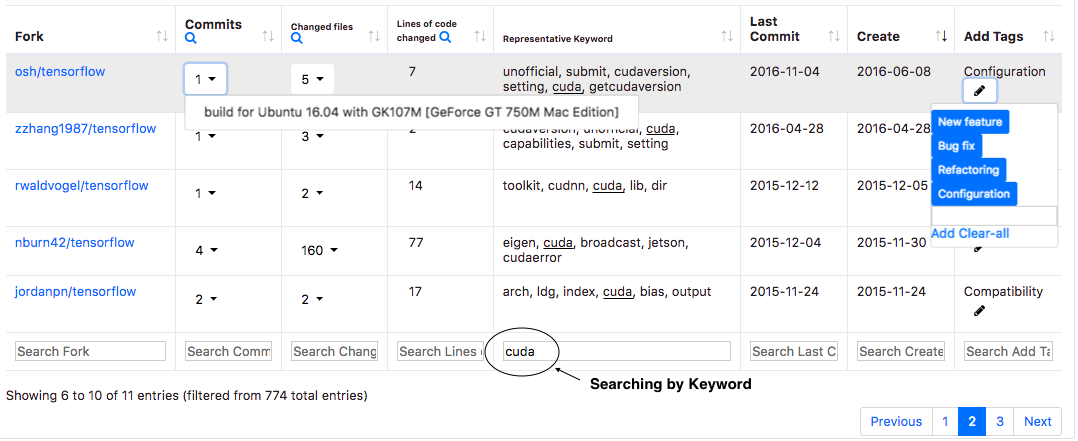
\includegraphics[scale=0.5]{tensorflow_cuda2.png}
\caption{User Interface of Forks Insight.\Luyao{more extra explaination here? and in picture?}}
\vspace{-6pt}
\label{GUI}
\end{figure*}

\subsection{Extracting Keywords}
To give developers a quick summary of what code changes have been made in each fork, we extract a list of representative keywords from text that are related to the code changes, such as source code, comments, and corresponding commit messages, by using the well-known natural language processing technique TF-IDF \cite{salton1988term}. Specifically, we first preprocess the text: removing all the numeric strings; splitting word into subtokens for Pascal Case and Camel Case; lemmatizing words into a normal form. Then, we extract keywords from the text by calculating TF-IDF weight of each token. Though TF-IDF could effectively filter out some stop words like "or", "and", there are still some words with high weight like "public", "private" that are meaningless for code summary. To improve the result, we manually add a list of  reserved words for different programming languages as stop words.

\subsection{Tagging Forks}
%
Developers fork a repository for different reasons: adding new features, fixing bugs, and changing configuration, etc.~\cite{Mikkonen2011,Robles2012,dubinsky2013exploratory,stanciulescu2015forked}.
%
This information could help developers of interests quickly find the fork they want to explore.
%
Thus, Forks Insight allows users to tag each fork by the main activity based on their understanding.
(see the last column in Fig.~\ref{GUI}). \Shurui{TODO: modify the screen-shot, show different tags, something like Feature-IDE's tags.} 
 We hope user's input on tags could not only help themselves maintain and understand each fork, but also help the whole community, especially for the new users who are not familiar with this repository to get a better overview. The tagging result will also be useful for future research.
 
\subsection{Searching Related Forks}

The interviews we did for INFOX show that the problem of redundant development exists in forks. For example, a developer found another fork implemented a very simple one-function as they did several years ago, and he said ``\emph{I think they should use our code, there is great reason to use it.''} Another developer said: \emph{"I can see multiple forks are working on the similar problem. This one looks like it is adding [...] that I already added"} ~\cite{ZSLXWK:ICSE18}.

To identify redundant development, we design the functionality of keywords searching, which is a simple and practical way to find code changes that are modifying the same keyword. For example, in Fig.~\ref{GUI}, if developer search for "cuda", which is a common keyword related to GPU configuration in repository of \emph{tensorflow/tensorflow}, Forks Insight will return several forks that have made code changes related to ``cuda''. This example shows that, by using keyword searching, user could find similar forks and potentially reduce the redundant development.

\iffalse
\begin{figure}[H] 
\centering
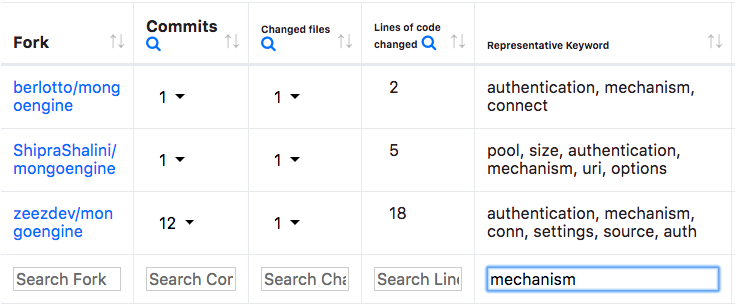
\includegraphics[scale=0.3]{shot2.png}
\caption{An example of searching for similar forks.}
\vspace{-10pt}

\end{figure}
\fi

\section{Conclusions and Future Work}
We implemented Forks Insight to help developers get an overview of forks. The current release version focuses on simple analytics for the high level overview which is lightweight, scalable and practical. it uses the keyword extraction of INFOX and extends We designed a user-friendly interactive web interface and features for searching and tagging. In order to improve the usability of Forks Insight, we plan to design a user study to ask for feedback from open source developers. And we would like to add more interactive elements and powerful functions into our tool. There are several directions we are considering to move forward: using more visualization to show meaningful data; identifying features in forks; summarizing the activities of forks by natural language.

\iffalse
\begin{acks}
  TODO
\end{acks}
\fi
